\documentclass[10pt] {article}
\usepackage[utf8]{inputenc}
\usepackage{amsmath}
\usepackage{graphics}
\usepackage{graphicx}
\usepackage[margin=2.5cm]{geometry}
\usepackage{color}
\usepackage{fancyhdr}
\usepackage{geometry}


% _____________________________________________________________________________________________________
\title{The Consistency Keys: A  Full Risk-Management System for Forex Trading}
\author{MR5OBOT \\ \textit{"It starts by hard work, but it's end with the smart work."}}
\begin{document}
\date{\today}
\maketitle
\pagestyle{fancy}
\tableofcontents 

% _____________________________________________________________________________________________________
\footnote{
  \textbf{\underline{Note:}}
  \small{This document is tailored for day traders, requiring basic math and trading knowledge for comprehension.}
}
\newpage
% _____________________________________________________________________________________________________
\section{The Missing Piece Of The Puzzle}
What has your Trading results shown you over the course of your career as a Trader? Are you struggling? Have you seen your account experience devastating drawdown or worse... blown it out? I purposely placed this topic at the beginning of the core material as I believe it is the most vital component to long term success in trading Forex... or any other asset class! I am confident the piece of the puzzle you are looking for is Risk Management. Have you risked more than 2\%\ of your total equity on any one trade? How about just about every one of them? Have you tried to over-leverage your account to make the losses back right away... only to find it resulted in steeper losses and deeper in depression? At the top of the list of crucial components to successful and consistent trading is the concept of Risk Management. Risk Management is basically divided into two core principles... Money Management and Trade Management. These areas are far greater in importance than your treasured little Trading System and patterns.

\vspace{0.3cm}
% _____________________________________________________________________________________________________
\begin{center}
  \textit{"Risk Management is your only shield against ultimate failure"}
\end{center}
% _____________________________________________________________________________________________________

\section{What Does Risk Management Really Mean?}
\subsection{Account Risk:}
This is the amount of Risk the Trader is willing to assume. It should be limited to 2\% of total equity or less. To calculate the Risk per trade use the following formula...

\begin{itemize}
    \item 
\end{itemize}

\vspace{11cm}
\noindent \textbf{\underline{Disclaimer:}}
\small{The content presented in this paper is provided for informational and educational pur-poses only and should not be considered as financial or investment advice. The author of this paper isnot a licensed financial professional, and the information contained herein should not be interpreted as a recommendation, endorsement, or solicitation to engage in any financial or investment activity. The views and opinions expressed in this paper are those of the author and do not represent the views of any financial institution, regulatory body, or other organization. The author assumes no responsibility for any financial losses, damages, or consequences resulting from the use of the information provided in this paper.}
% _____________________________________________________________________________________________________
\footnote{
  \textbf{Acknowledgment:} A special acknowledgment to Michael J. Huddleston, the ICT, for invaluable contributions to this document.}

\newpage
% _____________________________________________________________________________________________________

\begin{center}
\end{center}

\begin{figure}[h]
    \centering
    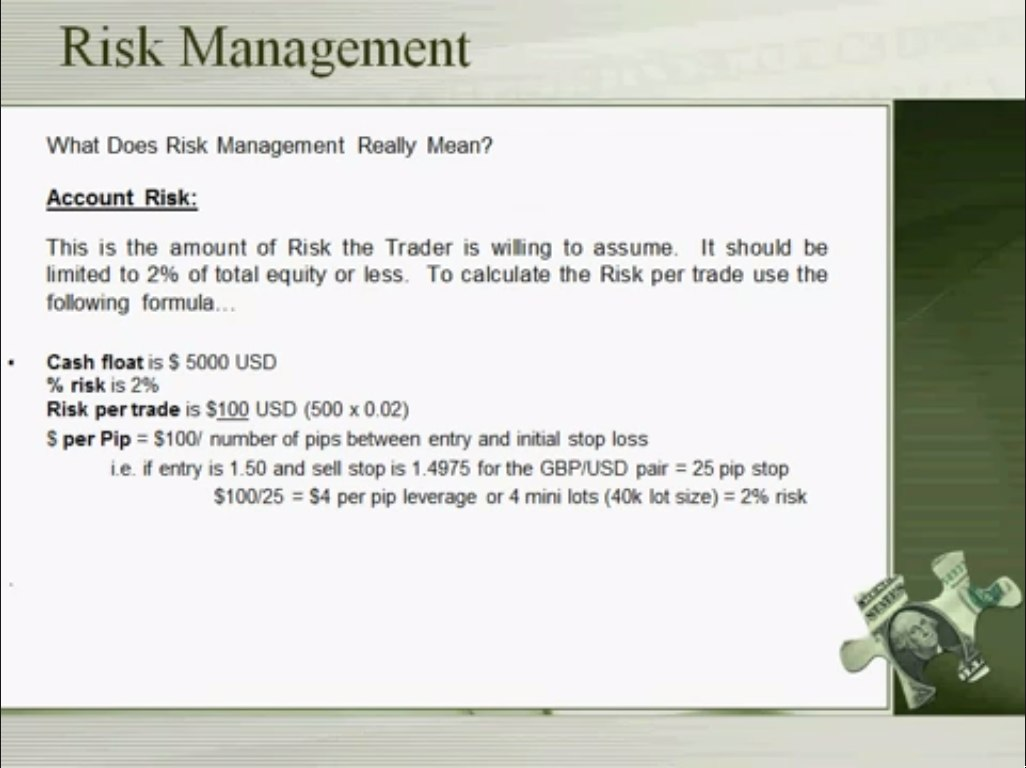
\includegraphics[width=1\textwidth]{./figures/Rsik_management.jpg}
    \caption{Risk-Management}
\end{figure}


\subsection{Money Management}
\subsection{Money Management Example}

\newpage
\section{Formulas}

\subsection{The combination of Risk-reward and Winrate} \vspace{0.8cm}

\[ \text{RR Formula}\ =\ \frac{\text{Win Rate}}{\text{1}\text{ - Win Rate}} \] \

\[ \text{Winrate Formula}\ =\ \frac{\text{Risk}}{\text{Risk} + \text{Reward}}\] \

 


\end{document}
